% ============================================================
% CHAPITRE II — ÉTAT DE L'ART
% ============================================================
\chapter{ÉTAT DE L'ART : APPROCHES INTELLIGENTES EN AGRICULTURE}

\section*{Introduction}
\addcontentsline{toc}{section}{Introduction}

L'agriculture moderne est confrontée à un double défi : augmenter les rendements tout en réduisant l'impact environnemental. En Tunisie, les pertes dues aux maladies végétales sont estimées entre 20\,\% et 40\,\% des récoltes~\cite{fao2021report}. L'absence d'outils de diagnostic précoce et accessible sur le terrain aggrave cette situation. L'intelligence artificielle, en particulier l'apprentissage profond appliqué à la vision par ordinateur et au traitement du langage naturel, ouvre des perspectives prometteuses.


Ce chapitre dresse un panorama critique des principales familles de modèles utilisables pour la détection des maladies végétales et l'assistance agricole. La première section présente les réseaux de neurones convolutifs (CNN), leur fonctionnement, leur évolution et leurs limites en conditions réelles. La deuxième section aborde les Transformers et les modèles vision-langage (VLM), qui intègrent des mécanismes d'attention et permettent l'interaction multimodale. La troisième section explore les techniques d'apprentissage adaptatif et dynamique: ensembles, few-shot, zero-shot et sélection dynamique, qui répondent aux contraintes d'évolutivité, de robustesse et d'hybridation Edge/Cloud. Une synthèse critique et le positionnement de l'architecture retenue pour le projet HydroNova concluent le chapitre.
\newpage
% ============================================================
\section{Réseaux de neurones convolutifs (CNN)}
\label{sec:cnnn}

\subsection{Principe général}
Les réseaux de neurones convolutifs (CNN) ont été conçus pour traiter efficacement des données structurées en grille, comme les images. Contrairement aux réseaux entièrement connectés, ils exploitent deux idées clés :

\begin{itemize}
	\item \textbf{Convolutions locales} : chaque neurone ne regarde qu'une petite région de l'image (son champ récepteur), ce qui réduit drastiquement le nombre de paramètres.
	\item \textbf{Partage des poids} : le même filtre (ou noyau) est appliqué sur toute l'image, ce qui rend le modèle invariant aux translations (un motif pathologique est reconnu où qu'il se trouve).
\end{itemize}

Une couche de convolution produit une \textit{carte de caractéristiques} (\textit{feature map}) qui met en évidence la présence de motifs élémentaires (contours, textures, taches). En empilant plusieurs couches, le modèle apprend des représentations de plus en plus abstraites : des arêtes dans les premières couches jusqu'aux structures sémantiques complexes (nécroses, lésions) dans les couches profondes. Des couches de \textit{pooling} (sous-échantillonnage) introduisent une certaine invariance aux petites déformations.


\subsection{Évolution des architectures CNN}
Le tableau~\ref{tab:cnn_archi} retrace les grandes étapes de l'évolution des CNN.

\begin{table}[htbp]
	\centering
	\small
	\begin{tabularx}{\textwidth}{|l|c|c|Y|}
		\hline
		\rowcolor[HTML]{2C3E50}
		\textcolor{white}{\textbf{Architecture}} & \textcolor{white}{\textbf{Année}} & \textcolor{white}{\textbf{ImageNet Top-1}} & \textcolor{white}{\textbf{Innovation clé}} \\ \hline
		AlexNet~\cite{krizhevsky2012imagenet} & 2012 & 63,3\,\% & ReLU, Dropout, parallélisation GPU. \\
		VGGNet-16~\cite{simonyan2014very} & 2014 & 74,4\,\% & Empilement de petits filtres 3×3. \\
		GoogLeNet~\cite{szegedy2015going} & 2015 & 74,8\,\% & Modules Inception (convolutions multi-échelles). \\
		ResNet-50~\cite{he2016deep} & 2016 & 76,1\,\% & Connexions résiduelles (\textit{skip connections}). \\
		InceptionV3~\cite{szegedy2016rethinking} & 2016 & 77,9\,\% & Factorisation des noyaux. \\
		MobileNetV2~\cite{howard2017mobilenets} & 2017 & 72,0\,\% & Convolutions séparables en profondeur (embarqué). \\
		EfficientNet-B4~\cite{tan2019efficientnet} & 2019 & 83,0\,\% & Mise à l'échelle coordonnée. \\
		ConvNeXt-T~\cite{liu2022convnet} & 2022 & 82,1\,\% & Modernisation inspirée des Transformers. \\ \hline
	\end{tabularx}
	\caption{Évolution des architectures CNN de référence}
	\label{tab:cnn_archi}
\end{table}

Les figures~\ref{fig:architecture-of-the-inceptionv3}, \ref{fig:ResNet-architecture} et \ref{fig:architecture-of-the-convnext} illustrent respectivement InceptionV3, ResNet et ConvNeXt.

\begin{figure}[h!]
	\centering
	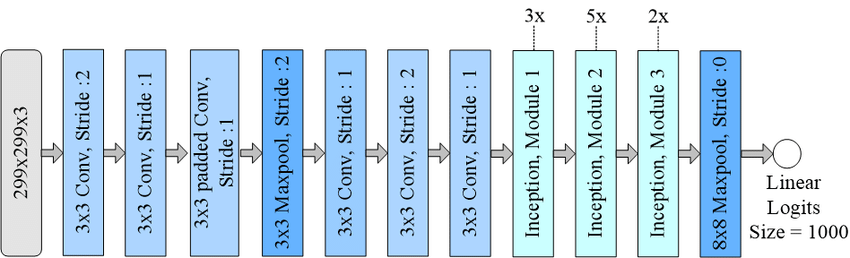
\includegraphics[width=0.7\linewidth]{public/Architecture-of-the-InceptionV3}
	\caption{Architecture d'InceptionV3 avec ses blocs parallèles.}
	\label{fig:architecture-of-the-inceptionv3}
\end{figure}

\begin{figure}[h!]
	\centering
	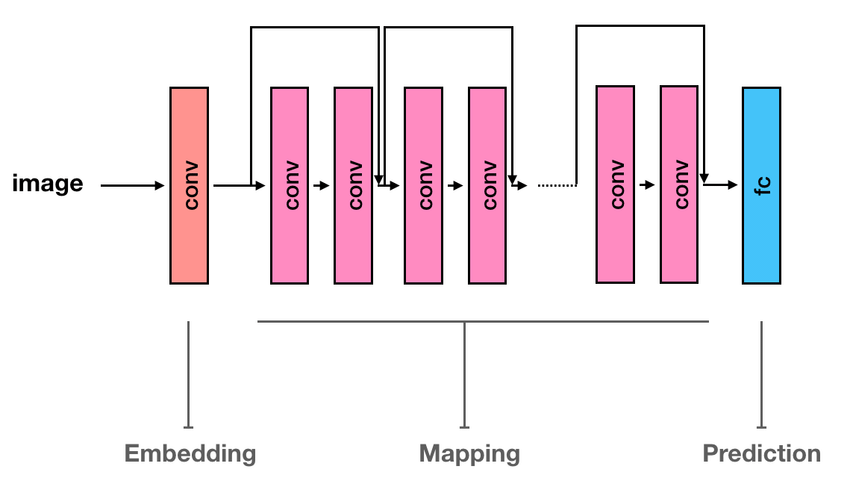
\includegraphics[width=0.7\linewidth]{public/resnetArchi}
	\caption{Architecture de ResNet (connexions résiduelles).}
	\label{fig:ResNet-architecture}
\end{figure}

\begin{figure}[h!]
	\centering
	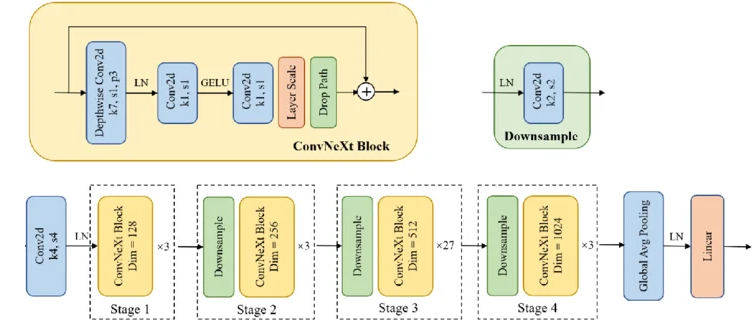
\includegraphics[width=0.7\linewidth]{public/Architecture-of-the-ConvNeXt}
	\caption{Architecture de ConvNeXt.}
	\label{fig:architecture-of-the-convnext}
\end{figure}
\newpage
\subsection{Limites des CNN pour le diagnostic agricole}
Les CNNs ont montré leur efficacité pour la classification de maladies sur des jeux de données comme \textit{PlantVillage}. Mohanty et al.~\cite{mohanty2016using} ont atteint une précision de 99,35\,\% pour 26 maladies sur 14 espèces. Too et al.~\cite{too2019comparative} ont comparé plusieurs architectures (VGG, ResNet, DenseNet) et conclu que les réseaux avec connexions résiduelles ou denses offrent une meilleure stabilité.

Cependant, des limites importantes apparaissent dès que l'on sort du cadre contrôlé du laboratoire~\cite{barbedo2018factors} :

\begin{enumerate}
	\item \textbf{Manque d'explicabilité} : un CNN donne une probabilité, mais ne peut expliquer son raisonnement (par exemple, sur quels pixels il s'appuie).
	\item \textbf{Information unidirectionnelle} : impossible d'intégrer des données contextuelles (historique de la culture, conditions climatiques) ou des questions de l'utilisateur.
	\item \textbf{Fragilité aux variations réelles} : changement d'éclairage, flou de bougé, chevauchement de feuilles dégradent fortement les performances.
\end{enumerate}

Ces lacunes motivent l'exploration d'architectures plus récentes, basées sur l'attention et la multimodalité.
% ============================================================
\section{Transformers et modèles vision-langage}
\label{sec:transformer_vlm}

\subsection{Le mécanisme d'attention et les Transformers}
Introduit pour le traitement automatique des langues~\cite{vaswani2017attention}, le mécanisme d'\textbf{auto-attention} permet à chaque élément d'une séquence d'interagir directement avec tous les autres, contrairement aux CNN qui ont une vision locale. Cette capacité à capturer des dépendances à longue distance est particulièrement utile en agriculture pour relier des symptômes distants sur une même plante. Les Transformers sont gourmands en données et en calcul, mais des variantes comme le \textbf{Swin Transformer}~\cite{liu2021swin} réduisent la complexité en limitant l'attention à des fenêtres locales.

\subsection{Grands modèles de langage (LLM)}
Les LLM (GPT, Gemini, etc.) sont des Transformers de type décodeur entraînés sur des masses de texte. Ils excellent en raisonnement et en génération de texte, mais sont \textbf{aveugles} : ils ne peuvent analyser une image. Pour le diagnostic agricole, ils doivent être combinés à un encodeur visuel.

\subsection{Modèles vision-langage (VLM)}
Un VLM associe trois composants : (1) un encodeur visuel (souvent un Vision Transformer), (2) un module d'alignement (projecteur ou Q-Former), (3) un LLM qui reçoit à la fois les tokens visuels et la question textuelle. Le tableau~\ref{tab:vlm_models} résume l'évolution récente.

\begin{table}[htbp]
	\centering
	\small
	\begin{tabularx}{\textwidth}{|l|c|Y|}
		\hline
		\rowcolor[HTML]{2C3E50}
		\textcolor{white}{\textbf{Modèle}} & \textcolor{white}{\textbf{Année}} & \textcolor{white}{\textbf{Innovation}} \\ \hline
		CLIP~\cite{radford2021learning} & 2021 & Apprentissage contrastif image-texte. \\
		BLIP-2~\cite{li2023blip2} & 2023 & Q-Former pour aligner vision et langage. \\
		LLaVA~\cite{liu2023llava} & 2023 & Projection linéaire + réglage par instructions. \\
		InstructBLIP~\cite{dai2023instructblip} & 2023 & Conditionnement du Q-Former par la question. \\
		\textbf{PaliGemma}~\cite{beyer2024paligemma} & 2024 & Architecture unifiée SigLIP + Gemma 2B. \\ \hline
	\end{tabularx}
	\caption{Évolution des modèles vision-langage}
	\label{tab:vlm_models}
\end{table}

La \textbf{question-réponse visuelle (VQA)} concrétise l'usage des VLM : l'utilisateur interroge le système en langage naturel, et le modèle répond en décrivant les symptômes (figure~\ref{fig:vqa-architecture}). Les VQA offrent une interaction guidée et une explicabilité, mais souffrent encore d'hallucinations, d'une forte dépendance au cloud, et d'une sensibilité aux conditions de prise de vue.

\begin{figure}[tbph]
	\centering
	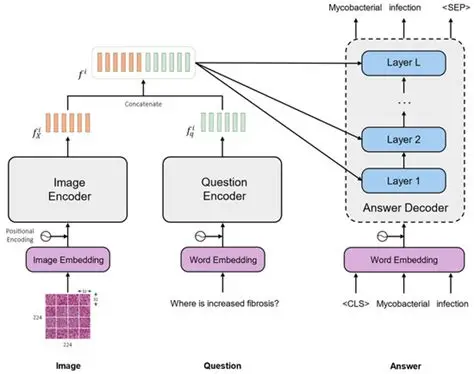
\includegraphics[width=0.7\linewidth]{public/vqa-architecture}
	\caption{Architecture fonctionnelle d'un système VQA.}
	\label{fig:vqa-architecture}
\end{figure}

\begin{figure}[tbph]
	\centering
	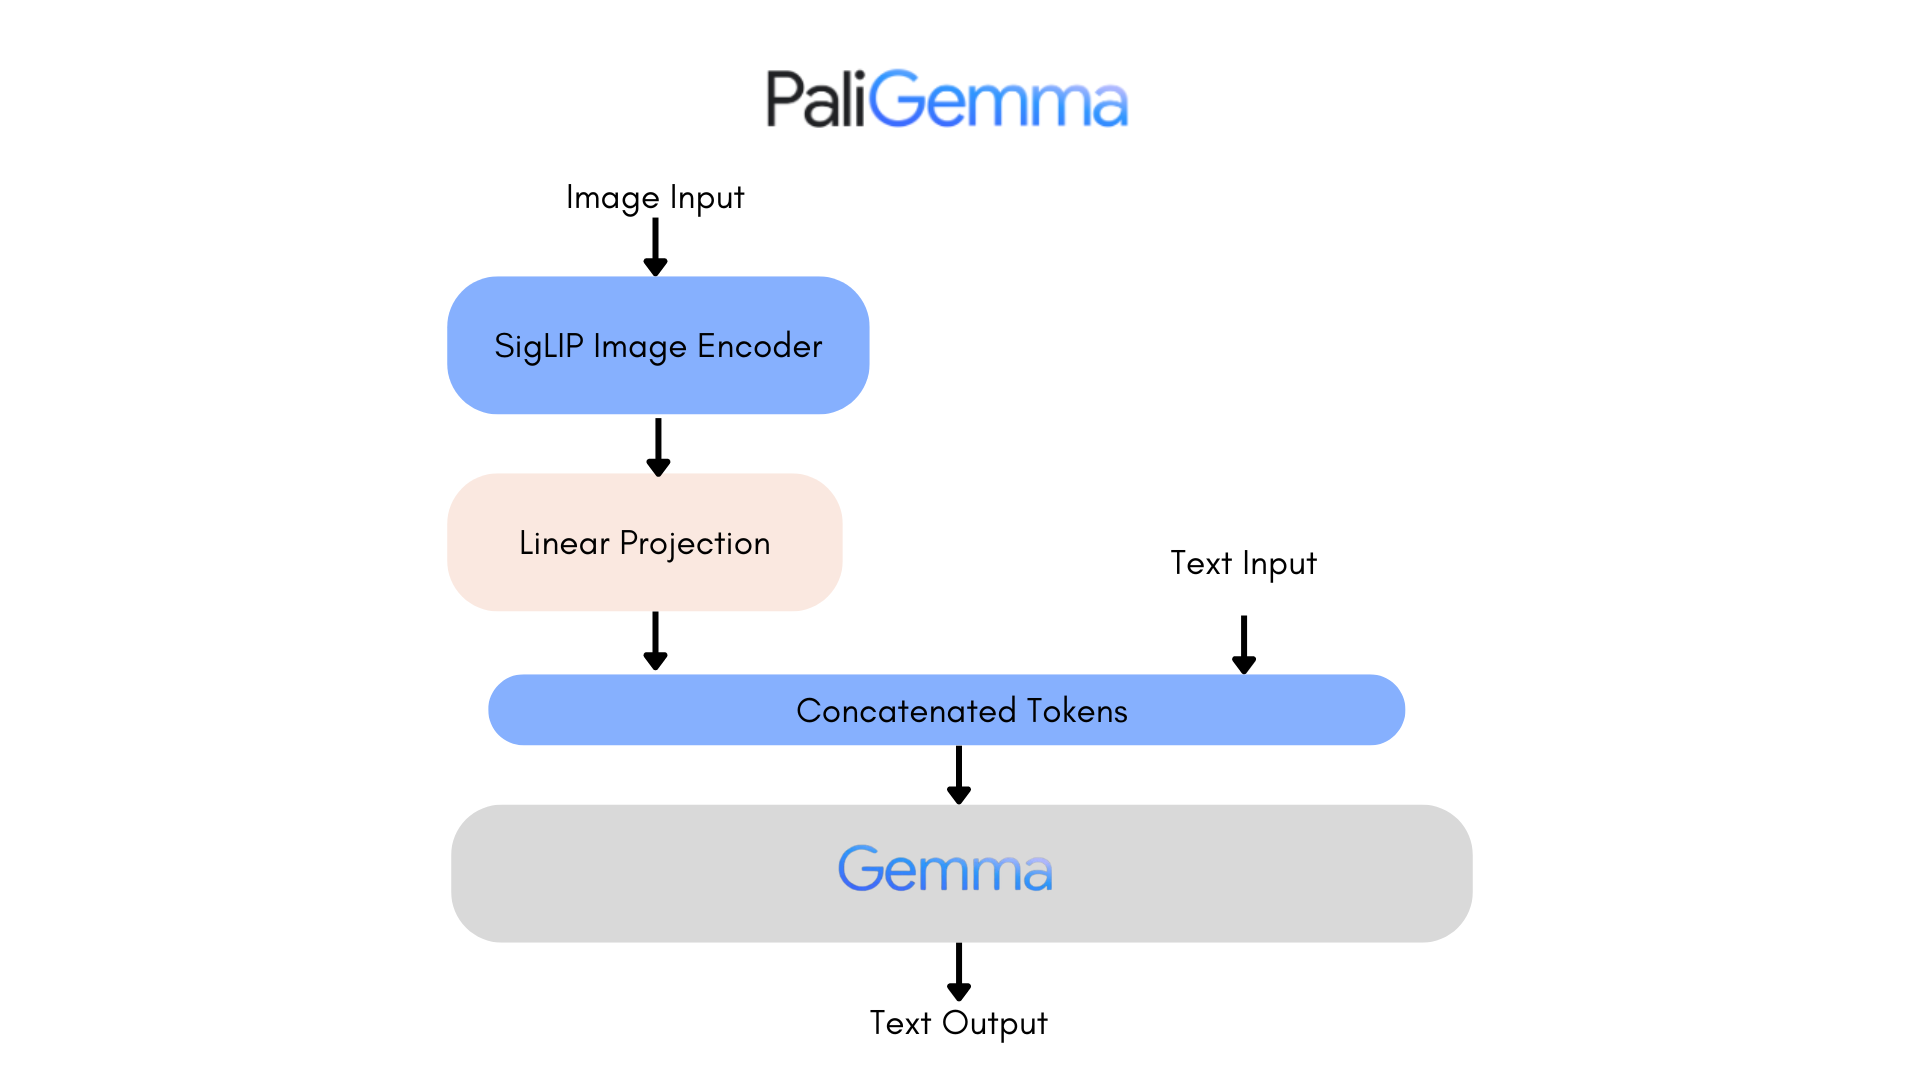
\includegraphics[width=0.7\linewidth]{public/paligemma_arch}
	\caption{Architecture de PaliGemma (SigLIP + Gemma).}
	\label{fig:paligemmaarch}
\end{figure}

% ============================================================

% ============================================================
\section{Apprentissage adaptatif et dynamique}
\label{sec:adaptive_dynamic}

L’agriculture de précision impose des modèles capables de s’adapter à des conditions changeantes (nouvelles maladies, variétés de plantes, environnements) tout en restant robustes et explicables. Cette section explore les techniques d’apprentissage qui permettent cette adaptabilité : les méthodes ensemblistes, l’apprentissage avec peu d’exemples (few-shot) et avec zéro exemple (zero-shot), ainsi que la sélection dynamique d’ensemble.

\subsection{Apprentissage par ensembles}
Les méthodes d’ensemble classiques, comme le \textit{bagging} (forêts aléatoires) ou le \textit{boosting} (AdaBoost, XGBoost), combinent plusieurs classifieurs pour réduire la variance et le biais. Appliquées aux réseaux de neurones, elles améliorent la robustesse : un ensemble de CNN peut surpasser n’importe lequel de ses membres pris isolément~\cite{dietterich2000ensemble}. Cependant, ces approches restent \textbf{statiques} : la combinaison des modèles est figée une fois l’entraînement terminé. Or, un modèle peut exceller sur certaines régions de l’espace des caractéristiques et être médiocre sur d’autres.

\subsection{Apprentissage avec peu d’exemples (few-shot)}
En environnement agricole réel, il est fréquent de devoir identifier une nouvelle maladie ou une variété végétale pour laquelle on ne dispose que de très peu d’images (parfois moins d’une dizaine). L’\textbf{apprentissage avec peu d’exemples} (few-shot learning) répond à ce besoin. Le \textbf{méta-apprentissage} (\textit{learning to learn}) en est une approche phare : l’algorithme MAML~\cite{finn2017model} apprend une initialisation des paramètres telle qu’une ou deux étapes de descente de gradient suffisent à adapter le modèle à une nouvelle tâche avec très peu de données. Cette capacité est cruciale pour un système comme HydroNova, qui doit pouvoir évoluer avec l’apparition de nouveaux pathogènes. D'autres approches comme \textit{Prototypical Networks}~\cite{snell2017prototypical} ou \textit{Relation Networks}~\cite{sung2018learning} sont également utilisées en agriculture~\cite{arguello2020few}.

\subsection{Apprentissage avec zéro exemple (zero-shot)}
Dans certains cas, aucune image de la nouvelle maladie n’est disponible au moment de l’entraînement. L’\textbf{apprentissage avec zéro exemple} (zero-shot learning) exploite des descriptions sémantiques (textuelles) des classes cibles. Les modèles vision-langage (VLM) comme CLIP~\cite{radford2021learning} ou PaliGemma sont naturellement adaptés au zero-shot : ils comparent l’image à une description textuelle de la maladie (par exemple, \textit{« taches brunes entourées d’un halo jaune sur feuilles de tomate »}) sans avoir jamais vu d’exemple visuel de cette pathologie. Cette approche est particulièrement pertinente pour les émergences phytosanitaires rapides~\cite{li2020zero}.

\subsection{Sélection dynamique d’ensemble (DES)}
Pour pallier le caractère statique des ensembles classiques, la \textbf{sélection dynamique d’ensemble} (DES) choisit, pour chaque image à classer, les modèles les plus compétents localement. Le framework \textbf{META-DES}~\cite{cruz2018meta} procède ainsi :
\begin{enumerate}
	\item Définition d’un voisinage de l’image cible (ses plus proches voisins dans un ensemble de validation).
	\item Extraction de \textit{méta-caractéristiques} pour chaque modèle candidat (précision locale, niveau de confiance, etc.).
	\item Prédiction par un méta-classifieur de la compétence du modèle pour cette image.
	\item Vote pondéré des seuls modèles jugés compétents.
\end{enumerate}
Cette approche améliore significativement la précision et la robustesse, particulièrement utile en milieu agricole où les conditions d’acquisition (éclairage, angle, chevauchement) varient fortement. Des travaux récents l'appliquent au diagnostic de maladies des plantes~\cite{zhang2020dynamic}.

\subsection{Pertinence dans le contexte agricole}
L’apprentissage adaptatif et dynamique répond à plusieurs contraintes du projet HydroNova :
\begin{itemize}
	\item \textbf{Évolutivité} : l’apparition de nouvelles maladies ou de nouvelles variétés de plantes peut être prise en compte via le few-shot ou le zero-shot, sans réentraînement complet.
	\item \textbf{Robustesse aux variations} : la sélection dynamique d’ensemble permet de s’adapter localement à des conditions de terrain changeantes.
	\item \textbf{Hybridation Edge/Cloud} : le few-shot et le zero-shot peuvent être déployés en cloud (via VLM), tandis que la sélection dynamique d’ensemble peut être embarquée sur le Raspberry Pi pour une inférence rapide hors-ligne.
\end{itemize}
Ces techniques complètent ainsi naturellement l’architecture hybride proposée : le module embarqué repose sur un ensemble dynamique de CNN (DES), tandis que le module cloud exploite un VLM capable de zero-shot et de few-shot.

% ============================================================
\section{Synthèse critique et positionnement}
\label{sec:synthese}

Le tableau~\ref{tab:synthese} compare les différentes familles de modèles selon des critères opérationnels.

\begin{table}[htbp]
	\centering
	\small
	\begin{tabularx}{\textwidth}{|l|X|X|c|c|}
		\hline
		\rowcolor[HTML]{2C3E50}
		\textcolor{white}{\textbf{Approche}} & \textcolor{white}{\textbf{Apports}} & \textcolor{white}{\textbf{Limites}} & \textcolor{white}{\textbf{Offline}} & \textcolor{white}{\textbf{Explicabilité}} \\ \hline
		CNN classiques & Efficaces, légers & Fragiles, boîtes noires & Oui & Faible \\
		Ensembles de CNN & Robustesse & Complexité & Oui & Faible/Moyenne \\
		Vision Transformers & Modélisation globale & Gourmands & Partiel & Moyenne \\
		LLM & Raisonnement, texte & Aveugles & Non & Élevée \\
		VLM / VQA & Multimodal, explicatif & Hallucinations, dépendance cloud & Non & Élevée \\
		Few-shot / Zero-shot & Adaptabilité rapide & Nécessite un pré-entraînement adapté & Partiel & Moyenne/Élevée \\
		DES (sélection dynamique) & Robustesse locale & Coût de calcul supplémentaire & Oui & Moyenne \\ \hline
	\end{tabularx}
	\caption{Synthèse comparative des paradigmes d'IA pour le diagnostic agricole}
	\label{tab:synthese}
\end{table}

Aucune approche unique ne satisfait toutes les contraintes du projet HydroNova : besoin d'un fonctionnement hors-ligne (serres isolées), de robustesse aux conditions réelles, d'évolutivité face à de nouvelles maladies, et d'explicabilité pour l'utilisateur.

C'est pourquoi nous proposons une \textbf{architecture hybride} articulant deux branches complémentaires :

\begin{itemize}
	\item Une branche \textbf{Edge} (embarquée sur Raspberry Pi) basée sur un ensemble dynamique de CNN (META-DES) pour une classification robuste, rapide et hors-ligne.
	\item Une branche \textbf{Cloud} exploitant un VLM (PaliGemma) pour l'assistance interactive, la génération d'explications, les cas ambigus, ainsi que l'adaptation en cas d'absence d'exemples.
\end{itemize}

Cette hybridation permet de concilier performance, résilience, adaptabilité et richesse sémantique.

% ============================================================
\section*{Conclusion}
\addcontentsline{toc}{section}{Conclusion}

Ce chapitre a présenté un panorama des principales architectures d'intelligence artificielle pour l'agriculture : CNN, Transformers, VLM, ainsi que les techniques d'apprentissage adaptatif et dynamique (ensembles, few-shot, zero-shot, sélection dynamique). L'analyse montre qu'aucun modèle isolé n'est suffisant, ce qui justifie l'approche hybride d'HydroNova. Le chapitre suivant détaille l'analyse des besoins et la spécification fonctionnelle du système.